\begin{frame}{\fe{3 Thermique linéaire}{3 Linear thermal analysis}}
             {\fe{Transitoire, conduction, convection, source}{Transient, conduction, convection, source}}
  \begin{itemize}
    \item \fe{Post traitement : boucle de tracés}{Post processing: loop for plot}
    \lstinputlisting[basicstyle=\ttfamily\tiny, language=gibiane, firstline=266, lastline=267]{dgibi/formation_debutant_2_thermique.dgibi}
    \lstinputlisting[basicstyle=\ttfamily\tiny, language=gibiane, firstline=271, lastline=276]{dgibi/formation_debutant_2_thermique.dgibi}
    \lstinputlisting[basicstyle=\ttfamily\tiny, language=gibiane, firstline=278, lastline=278]{dgibi/formation_debutant_2_thermique.dgibi}
    \lstinputlisting[basicstyle=\ttfamily\tiny, language=gibiane, firstline=280, lastline=280]{dgibi/formation_debutant_2_thermique.dgibi}
    \begin{textblock*}{5cm}(6.2cm,-1.4cm)
    \if \animation 1
      \animategraphics[controls,loop,poster=last,width=5.7cm]{10}{images/exo/3_temperatures.}{001}{101}
    \else
      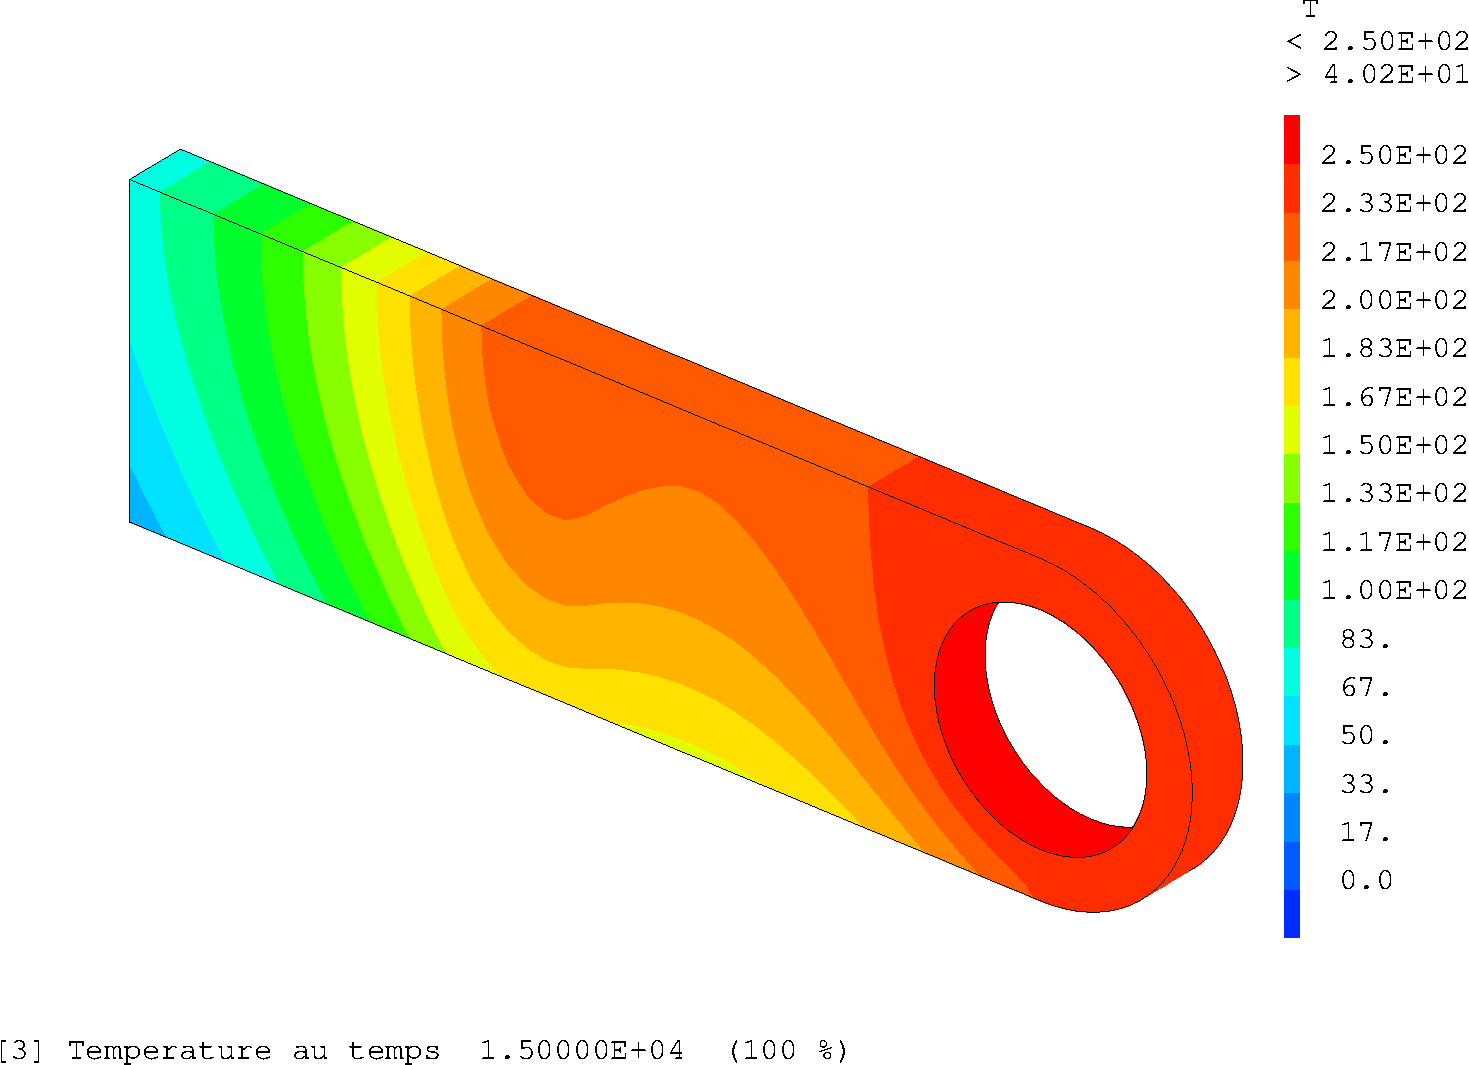
\includegraphics[width=5.7cm]{images/exo/3_temperatures.101}
    \fi
    \end{textblock*}
    \end{itemize}
    \vspace{3cm}
\end{frame}
